\chapter{Introducing Istio Security}
In a World that points towards cloud architectures and microservices-based applications, Istio seems the key to remove the strains from DevOps teams and simplify development, testing and observability. Indeed, it "lets you successfully, and efficiently, run a distributed microservice architecture, and provides a uniform way to secure, connect, and monitor microservices."\footnote{\href{https://istio.io/docs/concepts/what-is-istio/}{Istio's documentation}}.
One of the interesting aspects is related to \textit{how} Security is managed and \textit{how} the corresponding functionalities are really implemented. This chapter will be devoted to a general introduction of Istio Security, by analyzing the high-level architecture and some important keywords.

\minitoc

\vspace{0.5cm}
\section{High-level architecture}
Istio Security is designed in order to fulfill important microservices' security needs (e.g. access control, traffic encryption, fine-grained access policies, auditing tools) by exploiting \textit{security by default}, \textit{defense in depth}, and \textit{zero-trust network}.
Before examining in depth these concepts, it is necessary an high-level view of  Istio Security.

The general architecture comprises some key units:

\begin{itemize}
    \item \textbf{Pilot}: An \textit{API server}, that issues policies (for authentication and authorization) and other information to the proxies.
    \item \textbf{Citadel}: A \textit{Certificate Authority}, for key and certificate management.
    \item \textbf{Envoy}: Default proxy, Istio uses it to have \textit{Policy Enforcement Points} (PEPs), played by sidecar components and perimeter proxies, for channel security between clients and servers. 
    \item \textbf{Mixer}: Other \textit{Envoy proxy extensions} to manage telemetry and auditing.
\end{itemize}

That in the latest releases where consolidated in the \textbf{istiod} component in order to "simplifies mesh operability, while retaining Istio’s powerful functionality", as specified in the documentation. Furthermore, the releases 1.5 and 1.6 have introduced new Beta Authentication API that are workload-oriented, in contrast with the most used Alpha ones that is service-oriented. In this transient period, this project report will use both of them, depending on the particular example, trying to unify the Istio v1.4/v1.5/v1.6.

All those components are linked together to build the Istio Security architecture, showed in Fig.~\ref{fig:hlarch} (v1.6). The control plane interface manages configuration from the API server and configures the Policy Enforcement Points (Envoy) in the data level

\begin{figure}
    \centering
    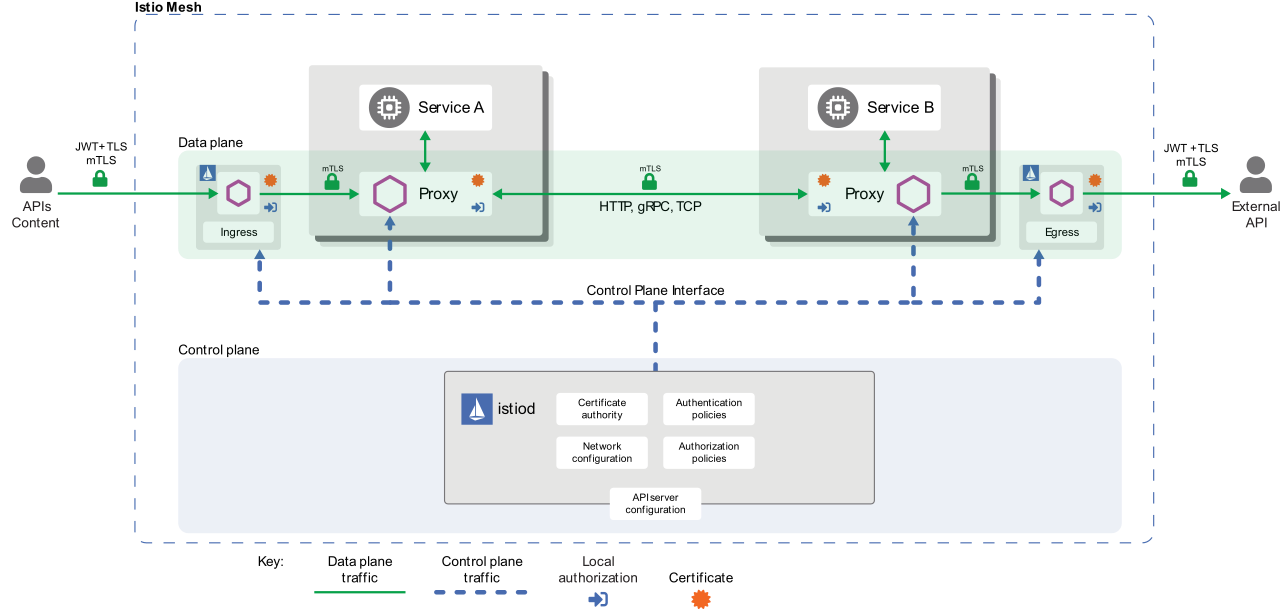
\includegraphics[width=0.9\textwidth]{chapters/images/chp1/arch-sec.png}
    \caption{Istio Security's high-level architecture, from Istio Docs}
    \label{fig:hlarch}
\end{figure}

\section{Identity and certificates}
After a very brief introduction on the big actors of Istio Security, in this section will be faced the common concepts of any security infrastructure: \textit{identity} and \textit{certificate management}.

\subsection{Istio Identity}
The mutual authentication forces the two components to exchange credentials with identity information when a workload-to-workload communication starts. At this point, both parts analyse the mutual identities in different manners: the client retrieves the secure naming information to see if the server is authorized to run the workload, while the server checks the authorization policies to ensure that the client has rights to access. 
In this last case, it is possible that the server charges clients based on the workload that they use or simply audit who accessed what and when.

The model of Istio Identity supports flexibility and granularity in order to represent an user, workload or groups of workloads using the \texttt{service identity} to resolve the identity of a request's origin.
There are several service identities available for different platforms: Kubernetes service account, AWS IAM role/user account and so on. A custom service account too is possible (on-premises).
\vspace{0.5cm}

\begin{figure}[ht]
    \centering
    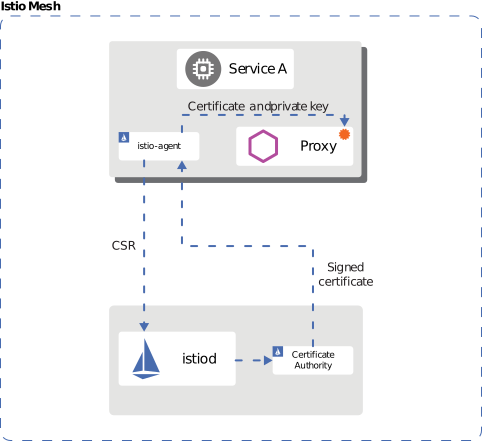
\includegraphics[width=0.5\textwidth]{chapters/images/chp1/cert-prov.png}
    \caption{Istio Security's identity provisioning flow, from Istio Docs}
    \label{fig:idprov}
\end{figure}

\subsection{Certificate management}
Istio Security supplies identities with X.509 certificates to every workload. In v1.6, the mechanism is supported by an \texttt{istio-agent} that runs alongside Envoy, assisted by the \texttt{istiod} service in order to automate the certificate rotation (Fig.~\ref{fig:idprov}).

It is clear that in a distributed and dynamic system, managing certificates and rotation can be quite time-consumig and error-prone when the clients are not all known in advance. \textit{Citadel} simplifies this process through a self-service model to establish end-to-end encryption (mTLS) between microservices by injecting certificates directly into them. Furthermore, it provides a self-signed root certificate and private key, which it uses to sign the workload certificates (a customer-supplied root certificate and key is also available).

In order to minimize exposure to compromised keys, the build-in \textit{Public Key Infrastructure} (PKI) generates certificates and automatically rotate keys.

\noindent The workflow is as follows:

\begin{itemize}
    \item[1.] A key and certificate request is sent by the Envoy proxy using the \textit{Secret Discovery Service} (SDS).
    \item[2.] Once the SDS request is received, the node's agent creates the private key and the \textit{Certificate Signing Request} (CSR).
    \item[3.] The CSR (with the key and credentials) goes through gRPC\footnote{From \href{https://grpc.io/}{gRPC Site}: "[...] a modern open source high performance RPC framework that can run in any environment."} directly to Citadel, that validates it, signs it, generates the certificate and resends is to the node agent.
    \item[4.] The node's agent sends key and certificate to the proxy through the SDS API. 
\end{itemize}

\noindent This process is repeated at a certain interval for each service for certificate/key rotation.



